\section{Description and event displays of high $\etmiss$ events} \label{EventDisplay}

\subsection{EB, spike at EB-EE boundary}
We see EB spikes occurring at the boundary between ECAL barrel and endcaps.

The ECAL spikes topological cuts employed in the calotower-based cleaning for tc$\etmiss$ 
are not currently applied to identify ``spikes'' candidates occurring at the boundary between ECAL barrel and endcaps. 
Spikes at the EB-EE boundary could anyway be removed by the timing cuts. Nevertheless, some of them still survives 
after the noise clean-up, as the event shown in Figure~\ref{fig:EBspikeAtBorder}.
It has been verified that all 22 spikes at EB-EE border reported in the tc$\etmiss$ scan are in fact reconstructed in-time, 
and therefore not removed.

All the observed EB spikes at EB-EE boundaries are instead cleaned by PF cleaning. 
The topological cuts applied at the EE/EB boundaries and in
the vicinity of intermodule cracks are tighter than elsewhere, such that they are 
as selective as in the fiducial ECAL region. 

\subsection{EB, EE spikes}
We see one event with an isolated spike in ECAL barrel (EB) far from the EB-EE boundaries 
(Figure~\ref{fig:EBEEspike}, left plot) and two events with an isolated spike in ECAL 
endcap (EE) (Figure~\ref{fig:EBEEspike}, right plot).

Calotower-based cleaning for spikes is not applied in EE (it is understood that 
spikes are due to particles hitting an APD, which are mounted only in the ECAL barrel). 
The case of EB spike, far from the EB-EE boundary and not cleaned, should be investigated.

All events are cleaned by PF; note that a topological cleaning for spikes is applied by default also in EE.

\subsection{HF, multi-PMT-hits or phi-strip events}
These events are characterized by several anomalous hits in adjacent cells; sometimes they show up as
a strip of hits at the same $i\phi$ location, as the ones reported in Figure~\ref{fig:HFmultiHits}. 
This type of noise cannot be cleaned by the existing topological algorithms but could 
be cleaned by the timing or pulse shape based 
cleaning if hits are out-of-time or have a malformed pulse shape. 
A topological cleaning based on the multiplicity of hits above certain energy threshold 
at the same $i\phi$ location might be effective at identifying such noise.
The source of such events is not yet fully understood.

Some of these events are identified by PF cleaning but not by calotower cleaning.
Such events are removed by PF cleaning mainly for two reasons:
\begin{itemize}
\item the use of the $E_S$/$E_L$-type variable also for long fibers (note: this cut, even being more aggressive on isolated photons 
than the S$9$/S$1$-type variable, it's still safe for physics thanks to the presence of the {\it a posteriori} recovery algorithm
implemented in PF cleaning);
\item the timing cleaning is first applied, and the topological cleaning is applied once 
the timing-cleaned hits are removed, making it efficient for multi hits as well.
\end{itemize}
%Studies are ongoing to understand the differences.

\subsection{HF, double-PMT-hits}
These events are characterized by significant energy in both long and short fibers in a single
isolated tower, as shown in Figure~\ref{fig:HFdoublehits}. For high $\etmiss$ events, 
this noise often shows up in the towers located at the smallest $\eta$ 
value in HF ($\eta$=3). This can be explained by the fact that, for a given energy, 
a noise occurring at smaller $\eta$ produces a larger transverse energy, and therefore is more visible at high $\etmiss$.
Anyway it's not excluded that double-hits occurs also at larger $\eta$; but in this case such events might 
fall in the bulk of $\etmiss$ distribution.

This type of noise cannot be cleaned by current calotower-based topological algorithms (PET or S9/S1) but can
be cleaned by the timing or pulse shape based cleaning if hits are out-of-time or have a malformed pulse shape.
However, cases of in-time double-hits with good pulse shape have been observed. In such cases, a cleaning based on
S$8$/S$1$ isolation variable could be effective, where S$8$/S$1$ is defined in a similar way to S$9$/S$1$
with the companion RecHit energy from the same HF tower left out from the sum. 
%On the other hand, this type of cleaning is not expected to be fully safe for isolated particles, 
%in particular for physically bigger towers at lower $\eta$ values. 
%Preliminary studies on the use of S$8$/S$1$ isolation variable have been performed. 

PF cleaning flags most of these noise events. 
The HF double-hits removed by PF cleaning are characterized by having 
energy in the short fiber larger than the energy in the long fiber. 
If, in addition to this condition, the HF tower is also isolated 
(i.e. small energy in the adjacent towers), the double-hit is identified by the PF cleaning algorithm.
No such algorithm is implemented for calotower cleaning in the release CMSSW\_3\_7\_0\_patch2; 
work ongoing to include it in CMSSW\_3\_8\_X.
%Studies are ongoing to understand the differences
%with calotower-based cleaning.

\subsection{HF, PMT hit embedded in a jet} ~\label{sec:HFHitEmbeddedInJet}
These events are characterized by one or more anomalous hits embedded inside a jet (or simply not isolated), 
as shown in Figure~\ref{fig:HFhitEmbeddedInJet}. This type of noise could arise from muons coming from 
in-flight decays of hadronic particles or from a jet punch-through. In both cases
such jets could be identified using the JetID variables since it is expected that a large fraction of the
total jet energy would come from only one or two HF towers. Due to an overlap between real and anomalous signal there are
two cleaning strategies possible: an entire event could be rejected or a more sophisticated anomalous energy
subtraction algorithm would have to be developed.

Neither calotower-based cleaning nor PF cleaning are able to identify these noise events 
(with the exception of one event removed by PF cleaning and not by calotower-based cleaning).

\subsection{HBHE, IonFeedback/HPD/RBX noise}
These events are characterized by low multiplicity noise or single noisy channels in HCAL barrel or endcap.
Two examples are shown in Figure~\ref{fig:HBHEnoise}.
Improved timing cuts could be employed to identify these residual noise events.

Neither calotower-based cleaning nor PF cleaning are able to identify these residual HBHE noise events.

\subsection{Physics}
It is observed that approximately 30\% of the high $\etmiss$ events don't contain an obvious source of noise
(and therefore are classified as ``Physics''). They are typically multi-jet events where 
the large fake $\etmiss$ is produced by jet energy mis-measurements or jets at the boundaries between sub-detectors, 
but can also be events with real $\etmiss$. Figure~\ref{fig:Physics} 
shows some examples of physics events with large $\etmiss$. 

In about 50\% of high tc$\etmiss$ events with multi-jet topology, pf$\etmiss$ values are 
smaller than tc$\etmiss$ values. More details can be found in 
the Tables~\ref{tab:tcMETskim} and ~\ref{tab:pfMETskim}, and in the list of events posted at the end of the note.
The events are classified based on the jet multiplicity using caloJets with uncorrected $p_T>10$~GeV.

\subsection{Others, large muon-induced pf$\etmiss$}
We observed 5 events with large pf$\etmiss$ (sometimes a few hundreds GeV) 
but very small tc$\etmiss$. 
The muon is reconstructed as ``global muon'' and ``standalone muon'', 
but not as ``tracker muon''. An example is shown in Figure~\ref{fig:largeMuonInducedPfMET}.

Info from PF group:

4 events with pf$\etmiss>80$~GeV, with pf$\etmiss$ = 83, 242, 337
and 528 GeV, respectively, and a muon with $|\eta| > 2.2$. 
These muons have all a central tracker track associated to them. They are
indeed not ``tracker muon'', meaning that they fail the tracker-muon
criteria, but they are all global muons (with a track and a stand-alone
muon part) for which the reco::muon pt is not correct. 
What is interesting is that such poorly reconstructed muons are not seen
in the simulation, which points to something odd in the muon and or
tracker alignment or geometry in this large eta region.

%
\begin{figure}[h]
 \centering
% \begin{tabular}{ll}
   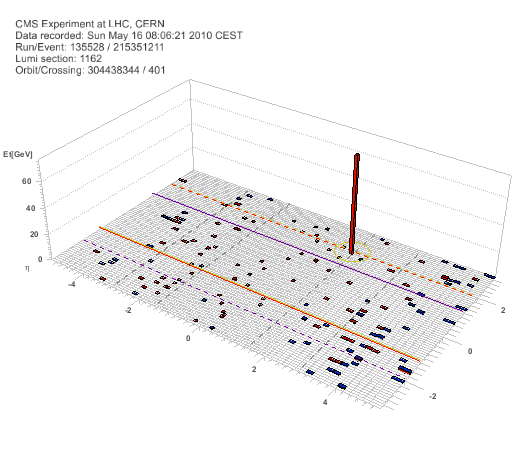
\includegraphics[width=0.47\textwidth]{fig/EBspikeAtBorder.png} 
% \end{tabular}
\caption{Example of an ``EB spike at EB-EE boundary'' event}
\label{fig:EBspikeAtBorder}
\end{figure}

%
\begin{figure}[h]
 \centering
 \begin{tabular}{ll}
   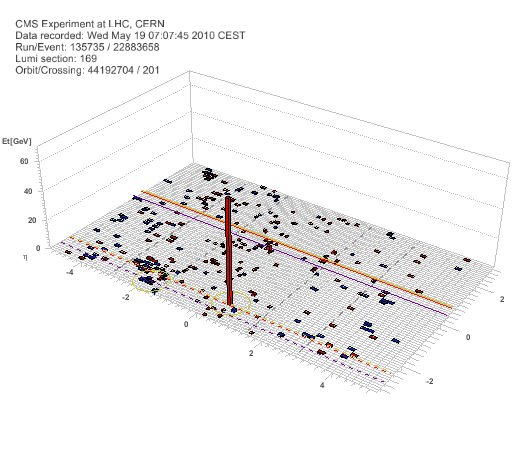
\includegraphics[width=0.47\textwidth]{fig/EBspike.png} &
   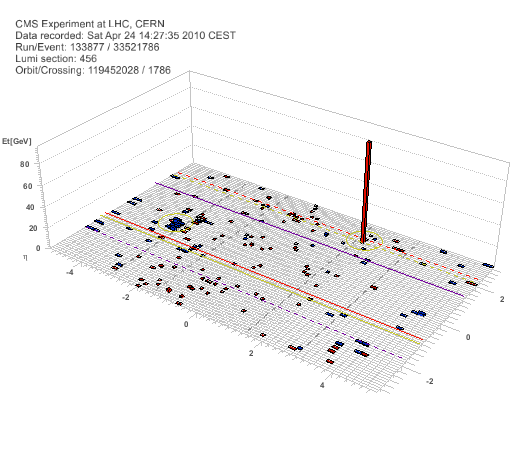
\includegraphics[width=0.47\textwidth]{fig/EEspike.png} \\
 \end{tabular}
\caption{Example of an ``EB spike'' (left) and an ``EE spike'' (right) event}
\label{fig:EBEEspike}
\end{figure}


%
\begin{figure}[h]
 \centering
 \begin{tabular}{ll}
   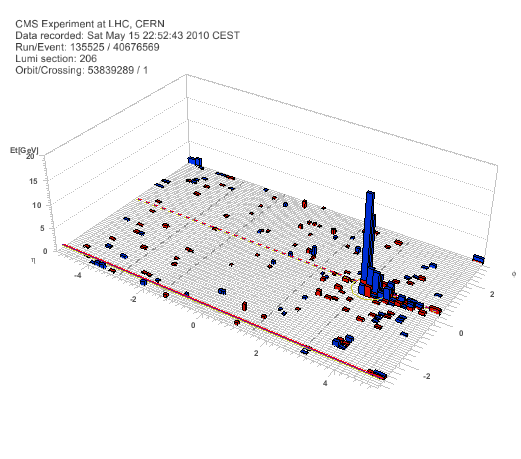
\includegraphics[width=0.47\textwidth]{fig/HFmultiHits.png} &
   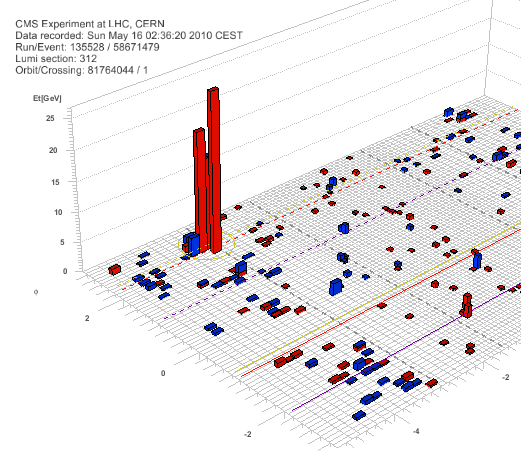
\includegraphics[width=0.47\textwidth]{fig/HFmultiHits_2.png} \\
 \end{tabular}
\caption{Example of two ``HF multi-PMT-hits or phi-strip'' events}
\label{fig:HFmultiHits}
\end{figure}

%
\begin{figure}[h]
 \centering
 \begin{tabular}{ll}
   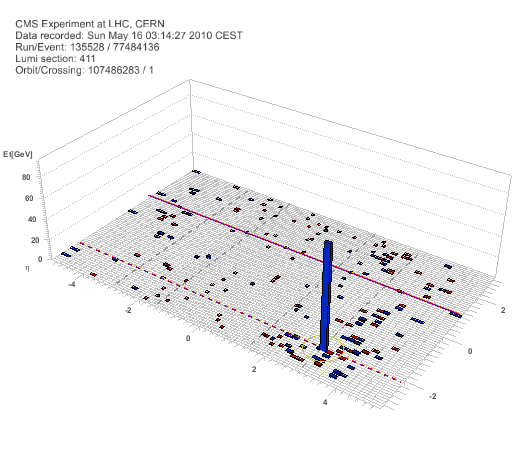
\includegraphics[width=0.47\textwidth]{fig/HFdoubleHit.png} &
   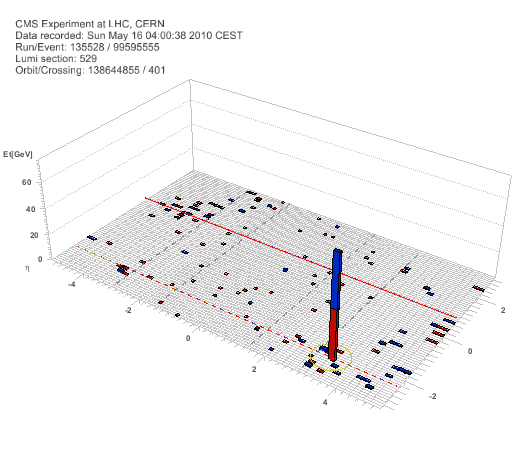
\includegraphics[width=0.47\textwidth]{fig/HFdoubleHit_1.png} \\
 \end{tabular}
\caption{Example of two ``HF double-PMT-hits'' events. Event in left plot is cleaned by PF and not by 
calotower-based cleaning; the event on the right is not cleaned by any of the two. 
NOTE: The event display for the left plot is mis-leading since the hit is not single, 
as it seems, but double. In fact, in this event display (produce with Fireworks) 
the following convention is used for HF towers: blue=2*$E_{S}$=hadEnergy, while red=$E_{L}-E_{S}$=emEnergy. 
In this event the emEnergy (``red'') is negative, but both energies in long and short fibers, $E_{L}$ and $E_{S}$, are large
(several hundreds of GeV). The event display only shows positive quantities 
(only the hadEnergy = ``blue''), so the ``negative'' red spike is not visible and it gives the illusion of a single hit. 
It is observed that most of double-hits cleaned by PF cleaning have negative emEnergy, i.e. $E_S>E_L$.}
\label{fig:HFdoublehits}
\end{figure}

%
\begin{figure}[h]
 \centering
 \begin{tabular}{ll}
   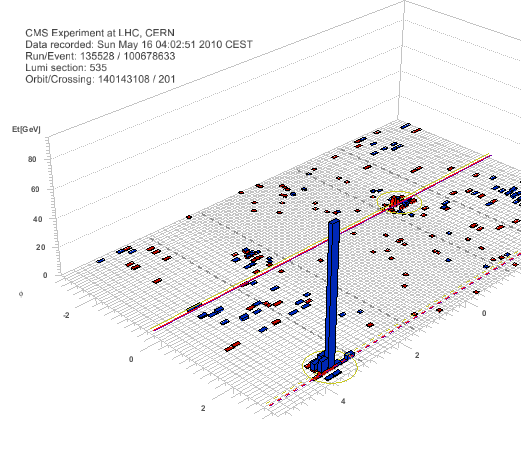
\includegraphics[width=0.47\textwidth]{fig//HFhitInJet.png} & 
   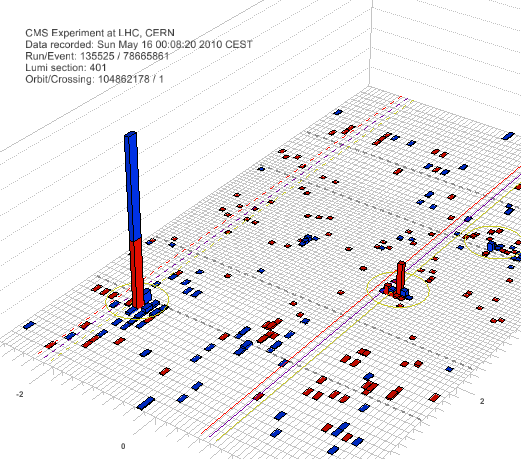
\includegraphics[width=0.47\textwidth]{fig//HFhitInJet_1.png} \\
 \end{tabular}
\caption{Example of two ``HF PMT hit embedded in a jet'' events}
\label{fig:HFhitEmbeddedInJet}
\end{figure}

%
\begin{figure}[h]
 \centering
 \begin{tabular}{ll}
   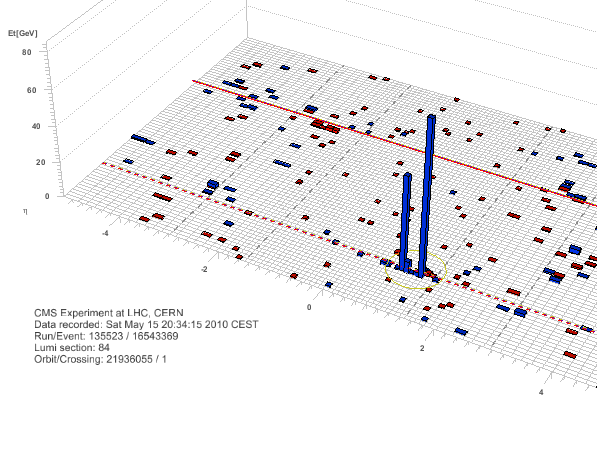
\includegraphics[width=0.47\textwidth]{fig/HBHEnoise_lowMult.png} &
   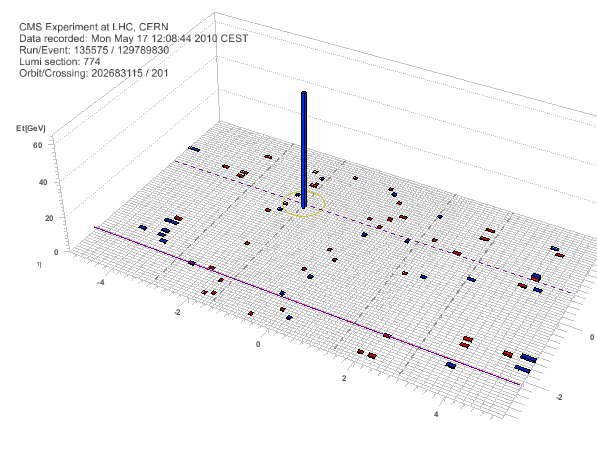
\includegraphics[width=0.47\textwidth]{fig/HBHEnoise_spike.png} \\
 \end{tabular}
\caption{Example of two ``HBHE IonFeedback/HPD/RBX'' noise events. 
The left plot shows an HPD/RBX noise event with low hit multiplicity. 
The right plot show instead an isolated spike, 
probably IonFeedback noise affecting an individual channel.}
\label{fig:HBHEnoise}
\end{figure}

%
\begin{figure}[h]
 \centering
 \begin{tabular}{ll}
   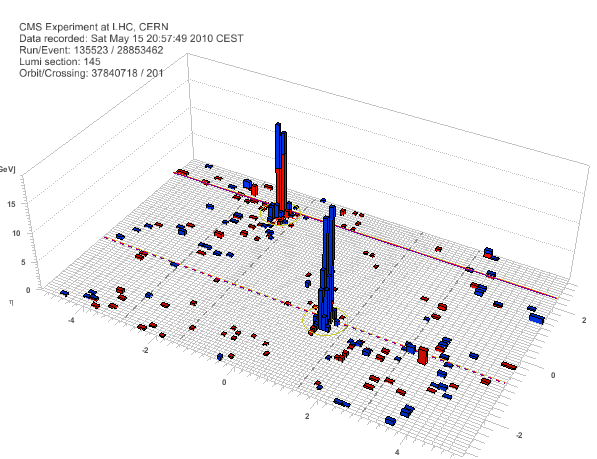
\includegraphics[width=0.47\textwidth]{fig/Physics2.png} &
   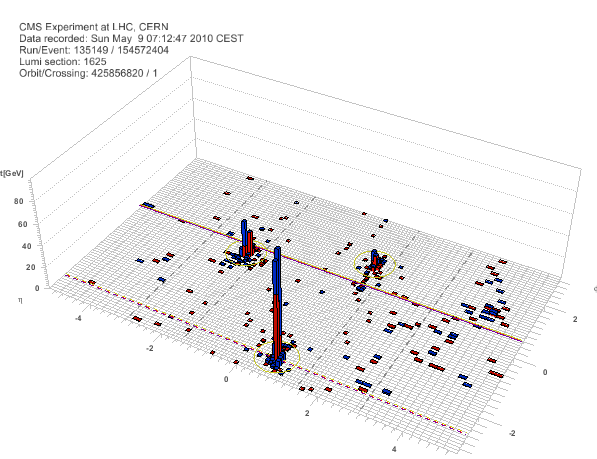
\includegraphics[width=0.47\textwidth]{fig/Physics3.png} \\
   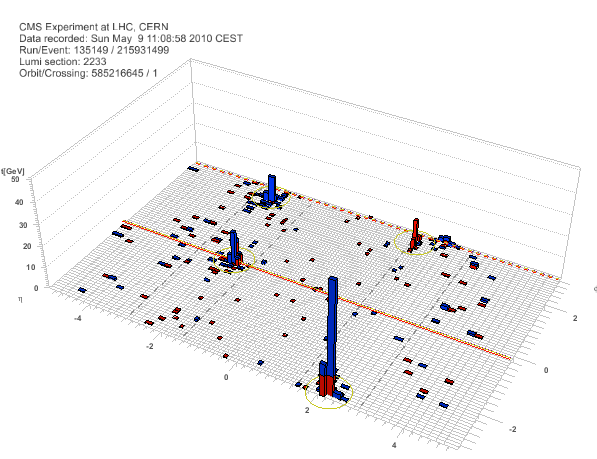
\includegraphics[width=0.47\textwidth]{fig/Physics4.png} &
   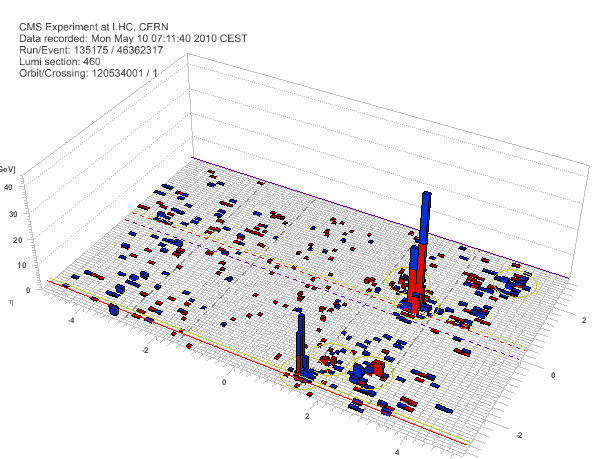
\includegraphics[width=0.47\textwidth]{fig/Physics6.png} \\
 \end{tabular}
\caption{Example of ``Physics'' events with multi-jet topology}
\label{fig:Physics}
\end{figure}

%
\begin{figure}[h]
 \centering
 \begin{tabular}{ll}
   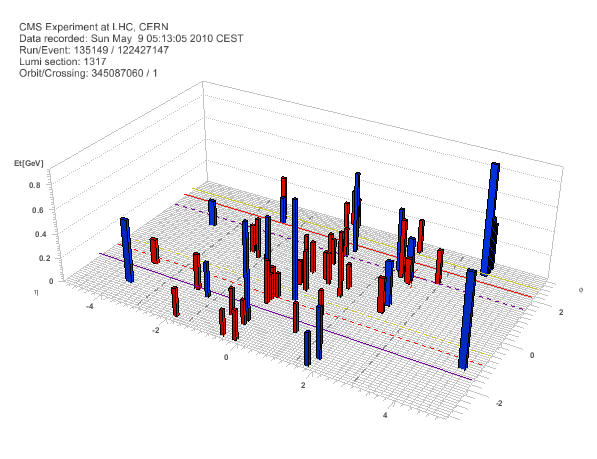
\includegraphics[width=0.47\textwidth]{fig/largeMuonInducedPfMET.png} &
   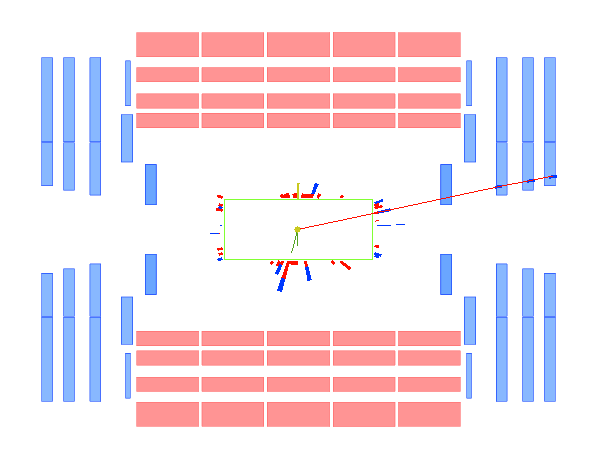
\includegraphics[width=0.47\textwidth]{fig/largeMuonInducedPfMET_1.png} \\
 \end{tabular}
\caption{Example of a ``large muon-induced pf$\etmiss$'' event
shown in the eta/phi view (left) and in the transverse plane view (right). There is an high $p_{T}$ 
muon reconstructed as ``global muon'' and ``standalone muon'' , but not as ``tracker muon''.}
\label{fig:largeMuonInducedPfMET}
\end{figure}




